% 3  Our work
% 3.1  Discuss our specific problem which allows us to apply spectral methods
% 3.1.1  Boundary condition: shore condition and ?wall? at some distance L
% 3.1.1.1  This is a potential problem we must keep track of? eta must be close to zero to avoid significant error.
% 3.1.2  Mention physical examples where ?wall? could exist
% 3.1.2.1  Actual physical wall-like object: dam, glacier, cliff, steep mountain, anything steep enough that does not move can be approximated as a wall
% 3.1.2.2  Point that the wave passes through but does not alter height (analogous to point in the middle of 2 standing waves)
%- 3.2  Go through spectral method for arbitrary m with Bessel solution.
% 3.3  Mention for m=2 this solution is simplified to sin solution
% 3.3.1  Still not fully analytic though because eigenvalues can only be found numerically


%3.11
\slide[Boundary Conditions]{
We chose to let:
\begin{align*}
\Phi_\sigma (0,\lambda)=0& ~ ~ ~ ~ \Phi_\sigma (L,\lambda)=0
\end{align*}
As $u(x,t)= \frac{1}{F(\sigma)} \Phi_\sigma(\sigma,\lambda)$
\[
u(x_{\sigma=0},t)=A(t) ~ ~ ~ \text{reflecting wall If wave does not break}
\]
and
\[
u(x_{\sigma_L},t)=0 ~ ~ ~ \text{Reflecting vertical wall}
\]
}
% 3.1.1.1
\slide[Potential Issue with BC's]{
We assume that $x_{\sigma_L}=const$ but

\[
x({\sigma_L},\lambda)=\frac{1}{2g\alpha}\left(  \Phi_\lambda(\sigma_L,\lambda)-2g H(\sigma_L)-\frac{1}{F(\sigma_L)}\Phi_\sigma(\sigma_L,\lambda)\right)
\]

}









% 3.2
	\begin{frame}
		\frametitle{IVBP}
			We wish to solve the following system:
			\begin{tabular}{l l l}
			\text{PDE: }& $\Phi_{\lambda \lambda}$&$=L\Phi$ \\\\
			\text{BC: }& $\Phi_\sigma (0,\lambda)$&$=0$\\
								 & $\Phi_\sigma (L,\lambda)$&$=0$\\\\
			\text{IC: }& $\Phi(\sigma,0)$&=$\int\limits_0^\sigma u_0(\sigma ')F(\sigma ')d \sigma'$\\
								 & $\Phi_\lambda(\sigma,0)$&=$2g\eta_0$\\
			\end{tabular}
			$\text{ where }L=\frac{\partial^2}{\partial \sigma^2}+\frac{m+1}{m\sigma}\frac{\partial}{\partial \sigma}$, $\sigma\in [0,\infty]$,and $\lambda\in [0,\infty)$
	\end{frame}
	
	
	
		\begin{frame}
		\frametitle{Solution Part 1}
				Assume solutions have the form $\Phi(\sigma,\lambda)=T(\lambda)X(\sigma)$.  We now have
				\begin{align*}
				\Phi_{\lambda \lambda}&=\left(\frac{\partial^2}{\partial \sigma^2}+\frac{m+1}{m\sigma}\frac{\partial}{\partial \sigma}\right)\Phi\\\\
				T''(\lambda)X(\sigma)&=T(\lambda)X''(\sigma)+\frac{m+1}{m\sigma}T(\lambda)X'(\sigma)\\\\
				\frac{T''(\lambda)}{T(\lambda)}&=\frac{X''(\sigma)}{X(\lambda)}+\frac{m+1}{m\sigma}\frac{X'(\sigma)}{X(\sigma)}\\
				\end{align*}
				So $T''(\lambda)=CT(\lambda)$ and $X''(\sigma)+\frac{m+1}{m\sigma}X'(\sigma)=C X(\sigma)$
	\end{frame}
	
	
	
	\begin{frame}
		\frametitle{Solution Part 2}
		 We now want to solve the system of ODEs:
		\[X''(\sigma)+\frac{m+1}{m\sigma}X'(\sigma)=C X(\sigma),\]
		\[T''(\lambda)=CT(\lambda)\]
		with conditions
		\[\Phi_\sigma (0,\lambda)=0\text{, }\Phi_\sigma (L,\lambda)=0\]
		\[ \Phi(\sigma,0)=\int\limits_0^\sigma u_0(\sigma ')F(\sigma ')d \sigma'\text{ and }\Phi_\lambda(\sigma,0)=2g\eta_0\]
	\end{frame}
	
	
	
	
		\begin{frame}
		\frametitle{Solution Part 3}
		 Letting $\alpha=\frac 1m$, $\varphi=X(\sigma)\sigma ^\alpha$, $t=\sigma \sqrt{C}$ and doing some algebraic manipulations we can rewrite 
		\[X''(\sigma)+\frac{m+1}{m\sigma}X'(\sigma)=C X(\sigma)\]
		as
		\[t^2 \varphi_{tt}+t \varphi_t-(\alpha^2+t^2)\varphi=0\]
		Which has well known solutions: the Modified Bessel Functions $I_\alpha(t)$ and $K_\alpha(t)$. Our solutions can be written as $$\varphi=C_1I_\alpha(t)+C_2K_\alpha(t).$$ We can also write our boundary conditions in terms of $\varphi$ as 
		\[\varphi(0)=0\text{ and }-\alpha\varphi(L\sqrt{c})+L\varphi'(L\sqrt{c})=0\]
	\end{frame}
	
	
	\begin{frame}
		\frametitle{Modified Bessel Functions}
		\centering
		\begin{tabular}{|c|c|}\hline
		$I_\alpha(t)$&$K_\alpha(t)$\\\hline
		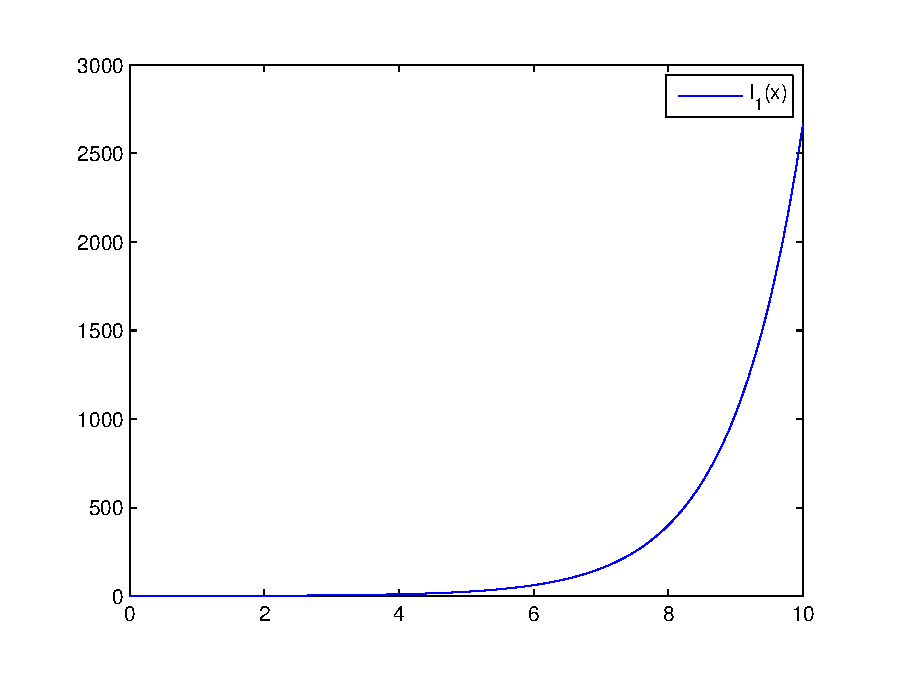
\includegraphics[width=.40\textwidth]{Bessel/BesselI.eps}&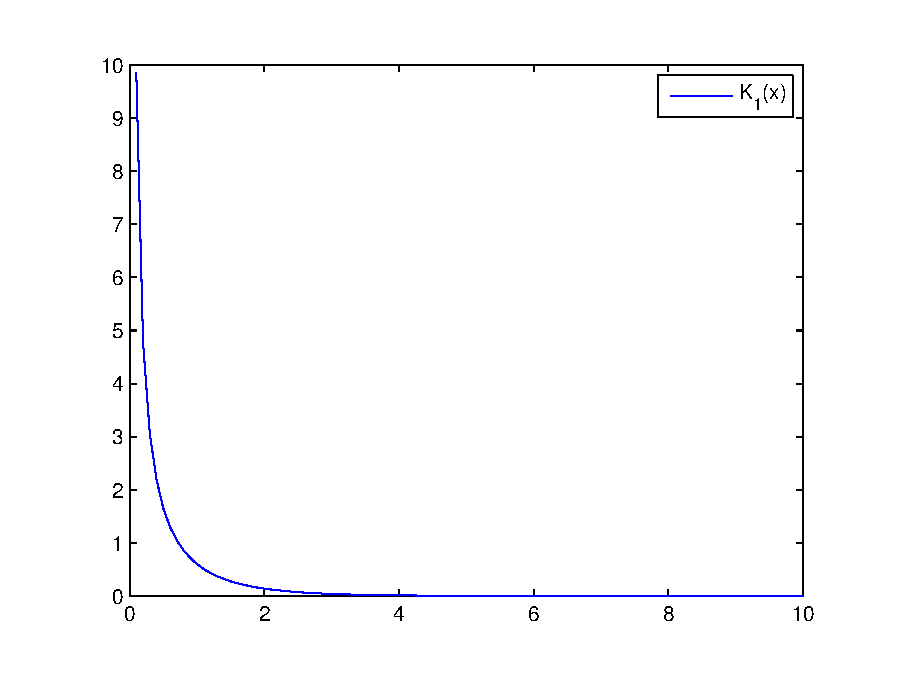
\includegraphics[width=.40\textwidth]{Bessel/BesselK.eps}\\\hline
		$J_\alpha(t)$&$Y_\alpha(t)$\\\hline
		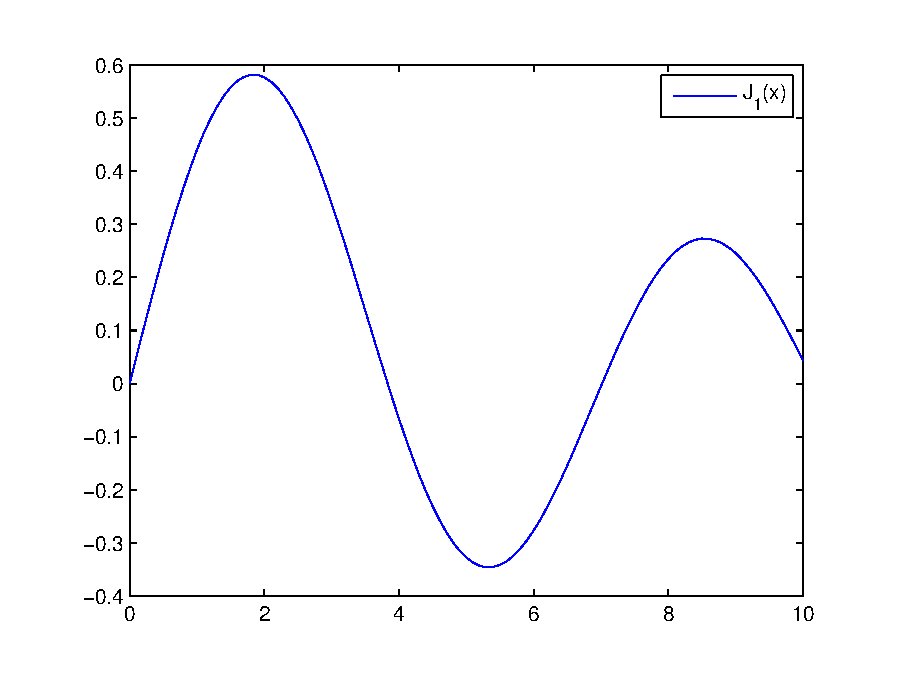
\includegraphics[width=.40\textwidth]{Bessel/BesselJ.eps}&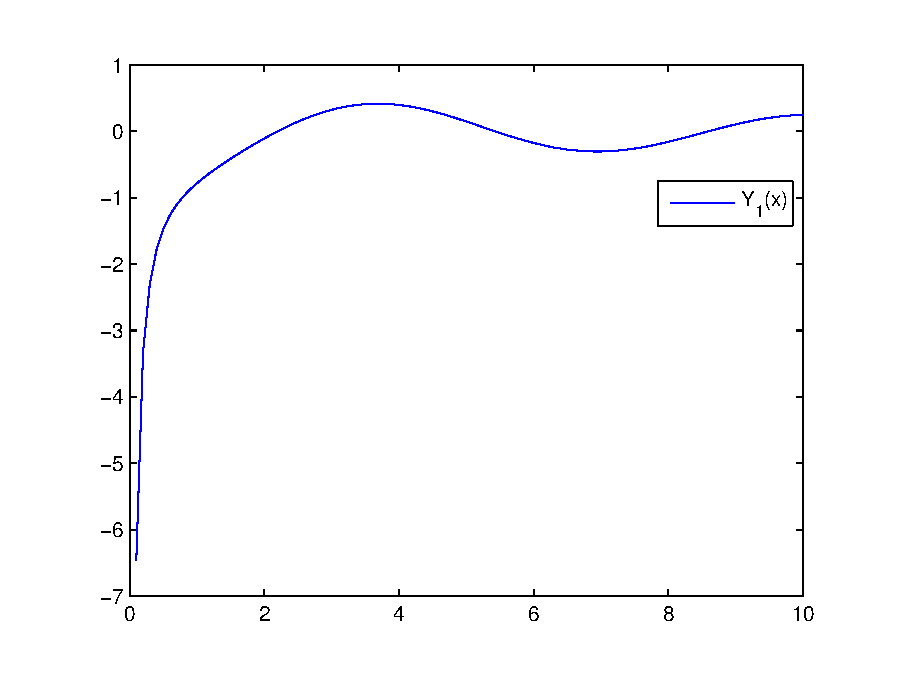
\includegraphics[width=.40\textwidth]{Bessel/BesselY.eps}\\\hline
		\end{tabular}\\
	\end{frame}
	
	
	
	
	
	
	
	
	
	\begin{frame}
		\frametitle{Solution Part 4}
		 We now conciser different values of $c$. We will only check the case where $c<0$ as the cases where $c=0$ and $c>0$ give trivial solutions.\\
		Letting $p=-c$, we can further 'simplify' $\varphi$ to 
		\[\varphi=D_1 i^\alpha J_\alpha(\sqrt{p}L)+D_2\left[\cot(\pi \alpha)-i^{-\alpha}Y_\alpha(L\sqrt{p})\right]\]
		Applying the first boundary condition we see that 
		\[0=D_1 i^\alpha J_\alpha(0)+D_2\left[\cot(\pi \alpha)-i^{-\alpha}Y_\alpha(0)\right]\]
		So $D_2=0$
	\end{frame}
	
	
	
		\begin{frame}
		\frametitle{Solution Part 5}
		 We now have $\varphi=D_1 i^\alpha J_\alpha(\sqrt{p}L)$. Using the second boundary condition gives
		\[
		D_1\left[-\alpha i^\alpha J_\alpha(L\sqrt{P})+Li^\alpha J'_\alpha(L\sqrt{p})\right]=0
		\]
		Simplifying we can write
		\begin{equation}
		J_{\alpha+1}(L\sqrt{p_n})=0\label{p}
		\end{equation}
		So our solutions for $\varphi$ are $\varphi=D_1i^\alpha J_\alpha(\sqrt{p_n}\sigma)$ where $p_n$ is a solution to \eqref{p}. Recalling that $\varphi=X(\sigma)\sigma ^\alpha$ we have
		\[
		X(\sigma)=\frac{J_\alpha(\sqrt{p_n}\sigma)}{\sigma^\alpha}
		\]
	\end{frame}
	
	
	
	\begin{frame}
		\frametitle{Solution Part 6}
		Recalling that our initial assumption was $\Phi(\sigma,\lambda)=T(\lambda)X(\sigma)$, we have
		\[
		\Phi(\sigma,\lambda)=\sum_{n=0}^\infty T_n(\lambda)\frac{J_\alpha(\sqrt{p_n}\sigma)}{\sigma^\alpha}
		\]
		We now solve the second ODE for $T$. Recall that
		$$T''(\lambda)=-p_nT(\lambda)$$
		The solution is:
		\[T(\lambda)=C_n \sin(\sqrt{p_n}\lambda)+D_n\cos(\sqrt{p_n}\lambda)\]
		So
		\[
		\Phi(\sigma,\lambda)=\sum_{n=0}^\infty C_n\frac{J_\alpha(\sqrt{p_n}\sigma)}{\sigma^\alpha} \sin(\sqrt{p_n}\lambda)+D_n\frac{J_\alpha(\sqrt{p_n}\sigma)}{\sigma^\alpha}\cos(\sqrt{p_n}\lambda)
		\]
	\end{frame}
	
	
	
	
		\begin{frame}
		\frametitle{Solution Part 7}
		Finally we use the ICs to write
		\[
		\sum_{n=0}^\infty D_n\frac{J_\alpha(\sqrt{p_n}\sigma)}{\sigma^\alpha}=\int\limits_0^\sigma u_0(\sigma ')F(\sigma ')d \sigma'
		\] and
		\[
		\sum_{n=0}^\infty C_n\sqrt{p_n}\frac{J_\alpha(\sqrt{p_n}\sigma)}{\sigma^\alpha} =2g\eta_0
		\]
		 Our final solution is:
				\[
		\Phi(\sigma,\lambda)=\sum_{n=0}^\infty C_n\frac{J_\alpha(\sqrt{p_n}\sigma)}{\sigma^\alpha} \sin(\sqrt{p_n}\lambda)+D_n\frac{J_\alpha(\sqrt{p_n}\sigma)}{\sigma^\alpha}\cos(\sqrt{p_n}\lambda)
		\]
		Where $J_{\alpha+1}(L\sqrt{p_n})=0$.
	\end{frame}
	
	
		\begin{frame}
		\frametitle{Numerical Implementation}
		To efficiently find the coefficients in the numerical code we solve the matrix systems
		\[
		\begin{pmatrix}
		\frac{J_\alpha(\sqrt{p_1}\sigma_1)}{\sigma_1^\alpha}&\ldots &\frac{J_\alpha(\sqrt{p_m}\sigma_1)}{\sigma_1^\alpha}\\
		\vdots&\ddots&\vdots\\
		\frac{J_\alpha(\sqrt{p_1}\sigma_n)}{\sigma_n^\alpha}&\ldots&\frac{J_\alpha(\sqrt{p_m}\sigma_n)}{\sigma_n^\alpha}\\
		\end{pmatrix}\begin{pmatrix}D_1\\\vdots\\D_m\end{pmatrix}=\begin{pmatrix} \int\limits_0^{\sigma_1} u_0(\sigma ')F(\sigma ')d \sigma'\\\vdots \\\int\limits_0^{\sigma_n} u_0(\sigma ')F(\sigma ')d \sigma' \end{pmatrix}
		\]
		and
				\[
		\begin{pmatrix}
		\frac{\sqrt{p_1}J_\alpha(\sqrt{p_1}\sigma_1)}{\sigma_1^\alpha}&\ldots &\frac{\sqrt{p_m}J_\alpha(\sqrt{p_m}\sigma_1)}{\sigma_1^\alpha}\\
		\vdots&\ddots&\vdots\\
		\frac{\sqrt{p_1}J_\alpha(\sqrt{p_1}\sigma_n)}{\sigma_n^\alpha}&\ldots&\frac{\sqrt{p_m}J_\alpha(\sqrt{p_m}\sigma_n)}{\sigma_n^\alpha}\\
		\end{pmatrix}\begin{pmatrix}C_1\\\vdots\\C_m\end{pmatrix}=\begin{pmatrix} 2g\eta_1\\\vdots \\2g\eta_n\end{pmatrix}
		\]
	\end{frame}
	

	
	
	
	
	
	
	
	
	
	
	
	
	
	
	
	
	
	
	
	
	
	
	
	